\section{Emboss}

\begin{frame}
    \frametitle{Emboss\footnote{\url{http://faculty.ycp.edu/~dhovemey/spring2011/cs365/labs/lab6.html}}}

    \begin{itemize}
        \item Jeder Pixel $ p^{rgba}_{ij} $ wird mit oben-links liegendem Pixel $ p^{rgba}_{i-1j-1} $ verglichen \pause
        \item Die größte, absolute Differenz wird als Referenzwert genommen
        \item $ d_{ij} = max(|p^{r}_{ij} - p^{r}_{i-1j-1}|, |p^{g}_{ij} - p^{g}_{i-1j-1}|, |p^{b}_{ij} - p^{b}_{i-1j-1}|) $ \pause
        \item Die Werte der Channels für den neuen Pixel entsprechenden dem Referenzwert addiert mit 128 und beschränkt auf 0-255, der Alpha-Channel vom Ausgangspixel übernommen \pause
        \item $ p' = min(0, max(255, d_{ij} + 128)) $
    \end{itemize}
\end{frame}

\begin{frame}
    \frametitle{Emboss - Ergebnisse 1}

    \begin{itemize}
        \item dice.png
        \item 800 x 600
        \item 295 KB
    \end{itemize}

    \hfill
    \hrule
    \hfill

    \begin{figure}[H]
        \centering
    
        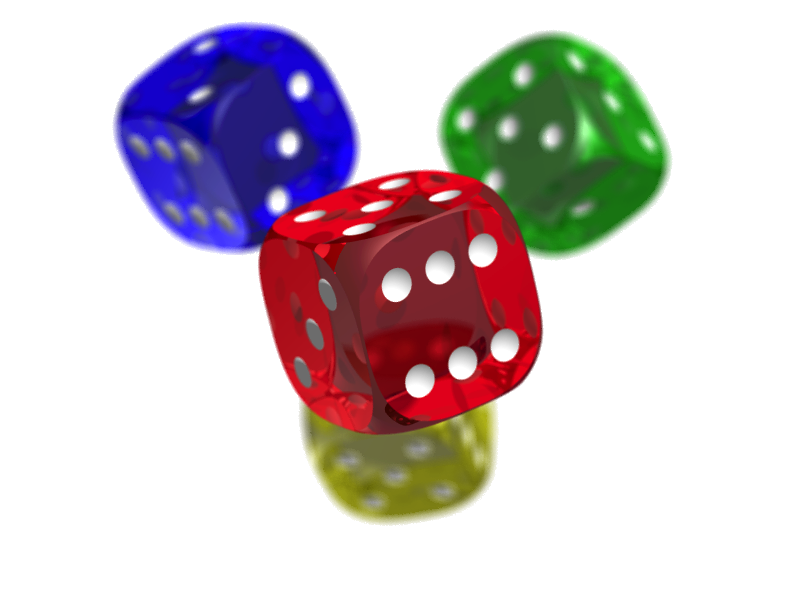
\includegraphics[width=0.30\textwidth]{images/dice.png}
        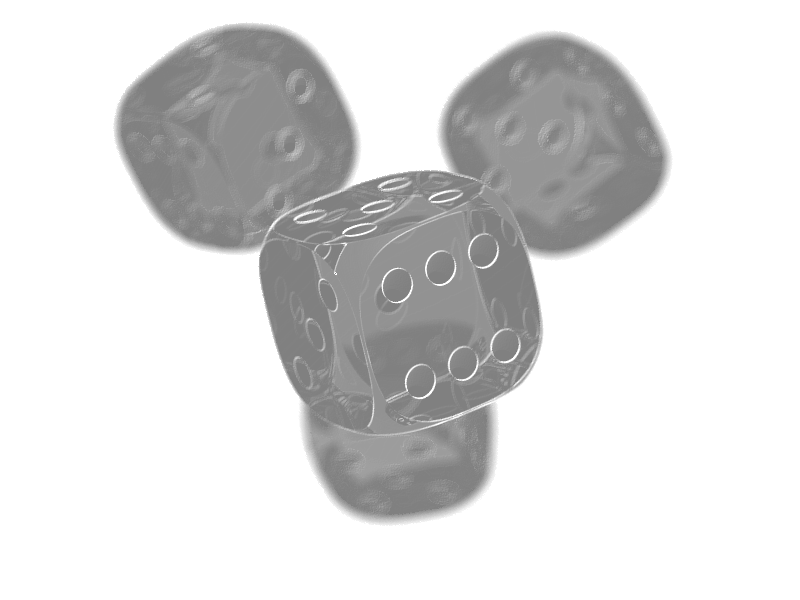
\includegraphics[width=0.30\textwidth]{images/results/emboss-my.dice.png}

        
        \begin{center}
            \caption{Emboss results of self-implemented Algorithm (right)}
        \end{center}

        \label{fig:emboss1}
    \end{figure}
\end{frame}

\begin{frame}
    \frametitle{Emboss - Performance 1}

    \begin{center}
    \begin{figure}[H]
        \centering

        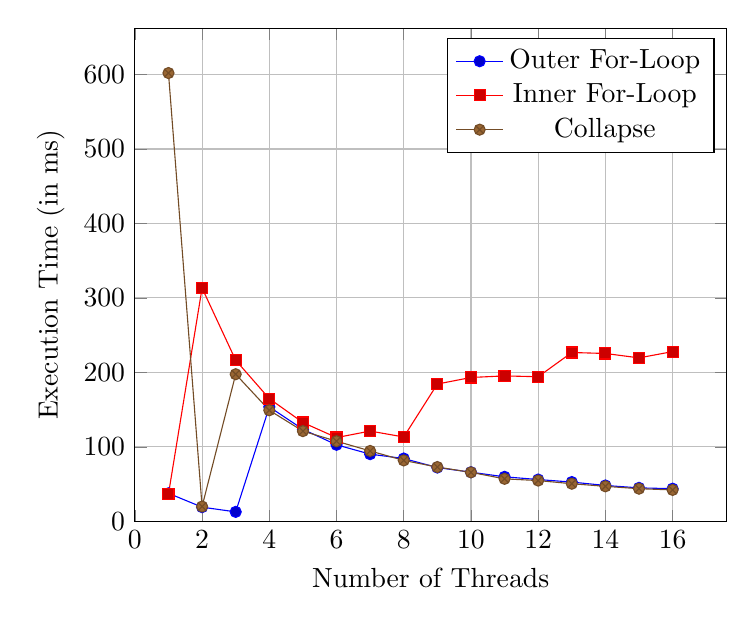
\begin{tikzpicture}
            \begin{axis}[
                title={},
                width=0.75\textwidth,
                xlabel={Number of Threads},
                ylabel={Execution Time (in ms)},
                xmin=0,
                ymin=0,
                grid=major
            ]
                \addplot coordinates {
                    (1,37.6192)(2,19.0143)(3,12.6701)(4,153.6)(5,123.528)(6,102.743)(7,90.193)(8,84.3286)(9,72.2025)(10,65.9573)(11,59.7616)(12,56.1131)(13,52.7063)(14,48.1298)(15,44.9207)(16,43.8277)
                };
                \addlegendentry{Outer For-Loop}

                \addplot coordinates {
                    (1,36.5978)(2,313.246)(3,216.304)(4,164.724)(5,132.658)(6,112.436)(7,121.197)(8,113.254)(9,184.333)(10,193.15)(11,195.278)(12,194.14)(13,226.703)(14,225.382)(15,219.47)(16,227.906)
                };
                \addlegendentry{Inner For-Loop}       

                \addplot coordinates {
                    (1,601.954)(2,19.8608)(3,197.528)(4,149.097)(5,121.117)(6,107.558)(7,94.5198)(8,81.7579)(9,72.864)(10,65.7456)(11,57.0341)(12,54.7264)(13,50.4797)(14,46.9844)(15,43.8079)(16,42.1596)
                };
                \addlegendentry{Collapse}
            \end{axis}
        \end{tikzpicture}
        \caption{Emboss Performance Tests dice.png}
    \end{figure}
\end{center}

\end{frame}

\begin{frame}
    \frametitle{Emboss - Ergebnisse 2}

    \begin{itemize}
        \item dice\_large.png
        \item 1754 x 1554
        \item 1.5 MB
    \end{itemize}

    \hfill
    \hrule
    \hfill

    \begin{figure}[H]
        \centering
    
        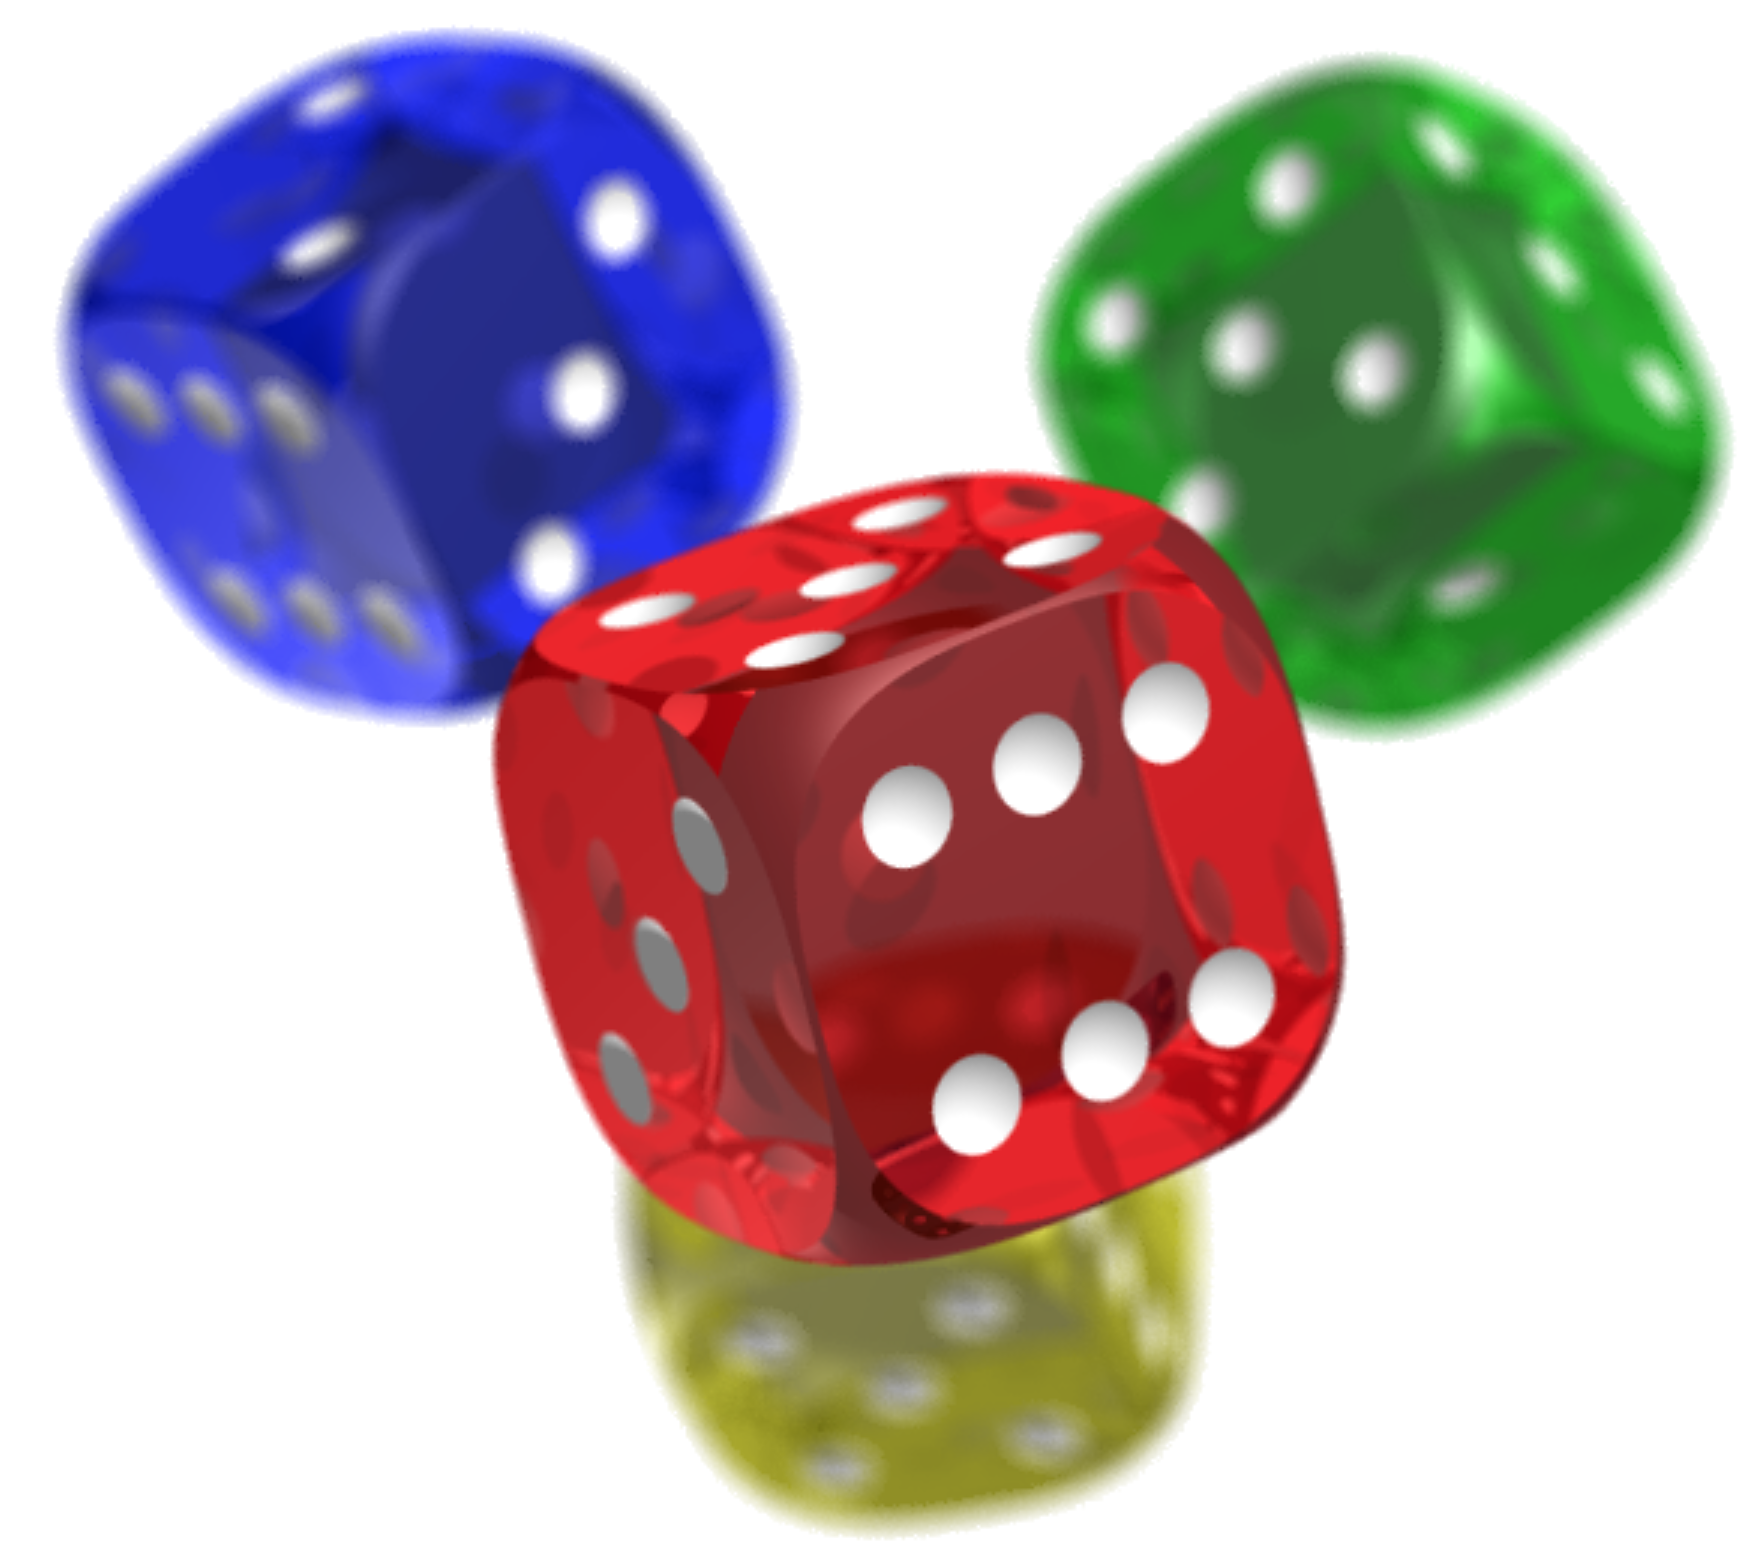
\includegraphics[width=0.30\textwidth]{images/dice_large.png}
        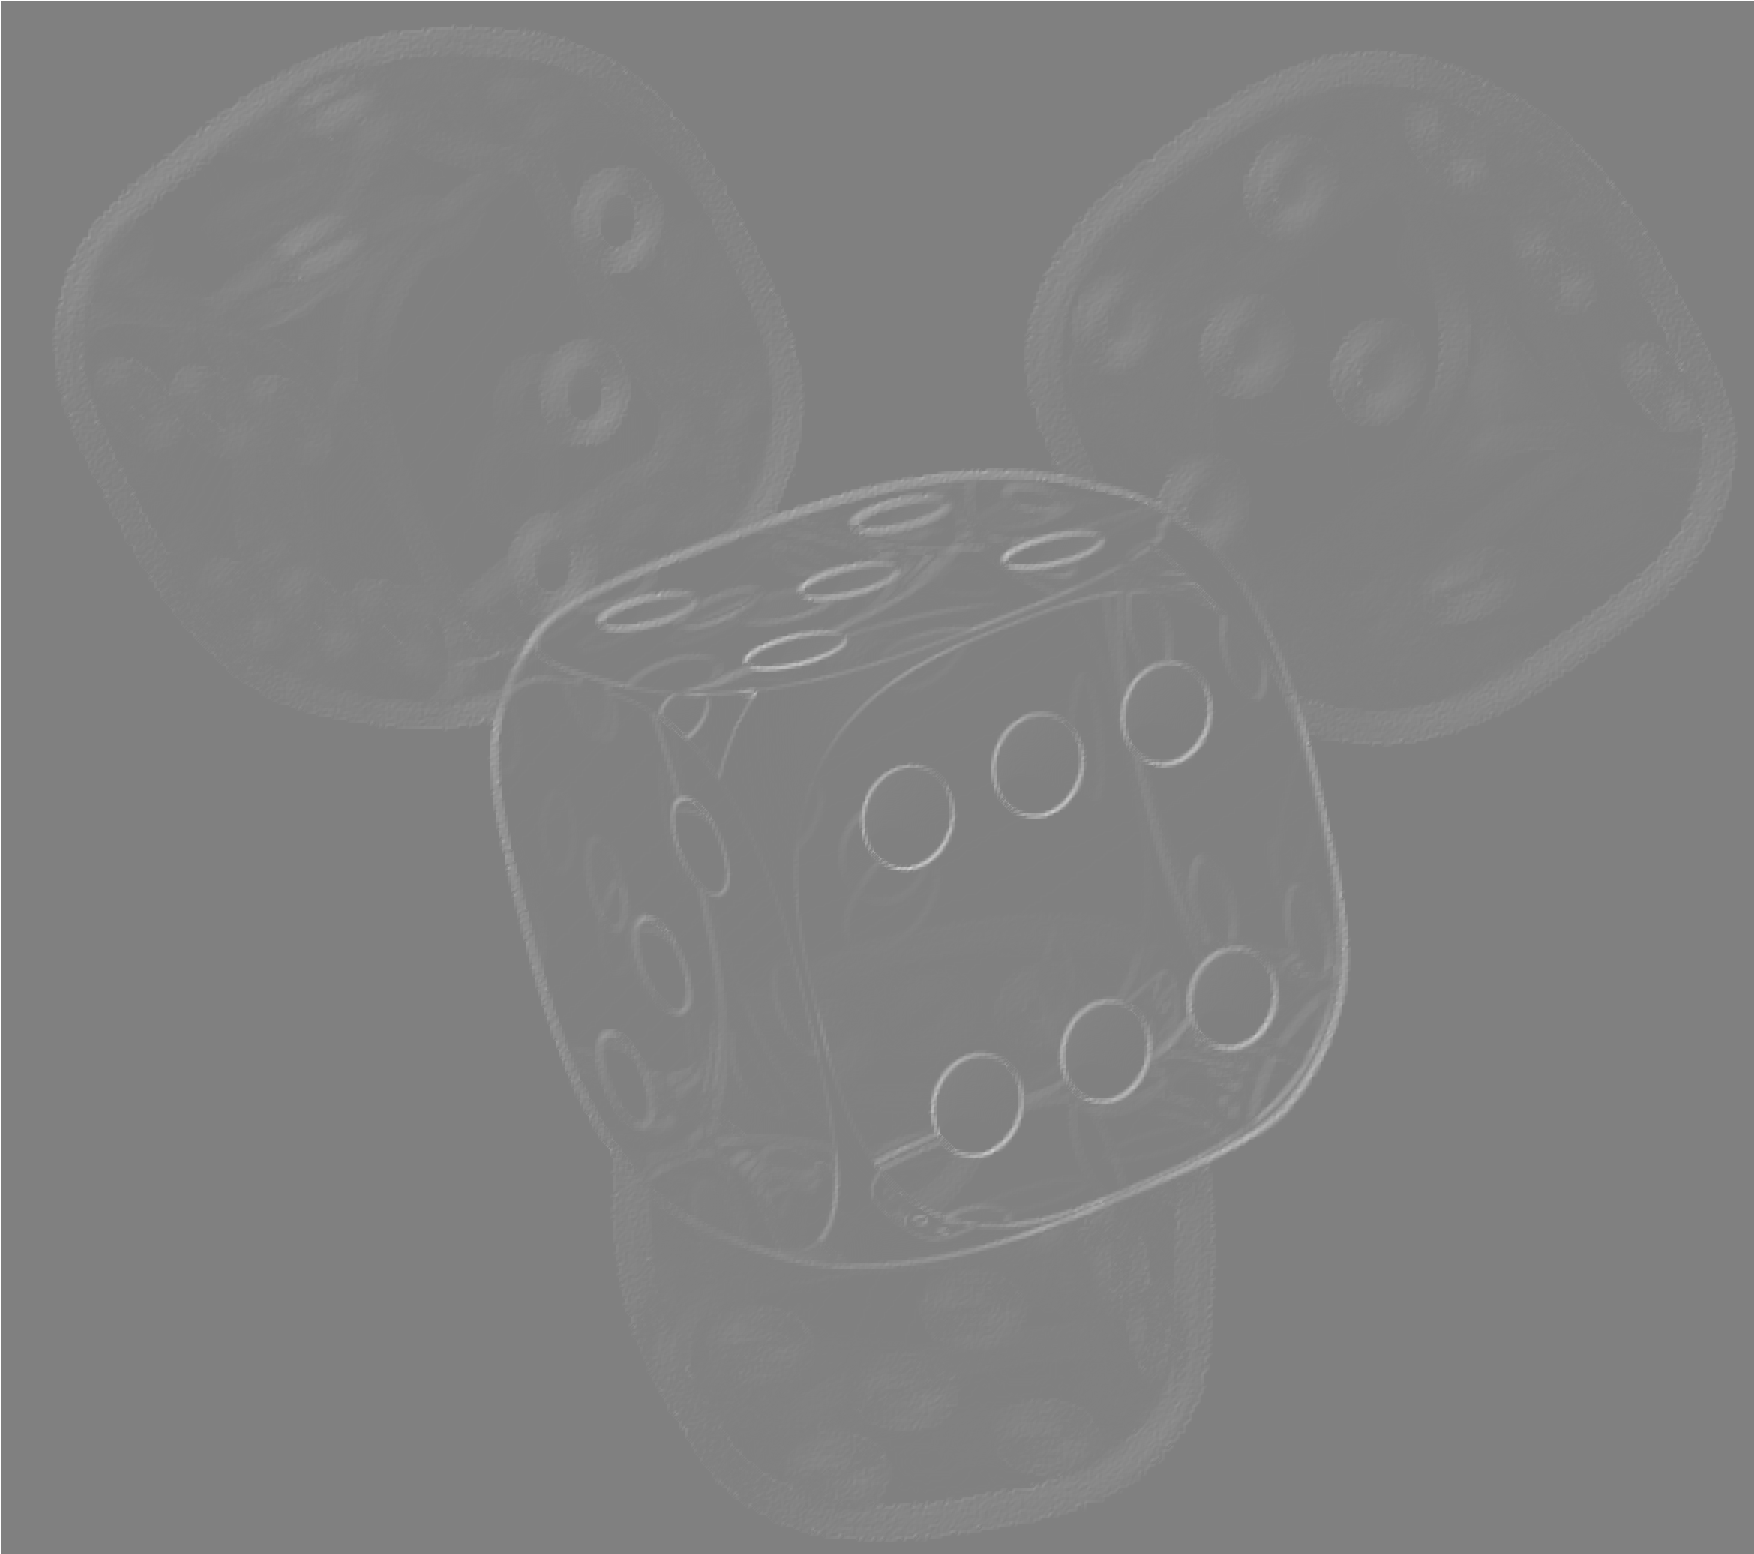
\includegraphics[width=0.30\textwidth]{images/results/emboss-my.dice_large.png}

        
        \begin{center}
            \caption{Emboss results of self-implemented Algorithm (right)}      
        \end{center}

        \label{fig:emboss2}
    \end{figure}
\end{frame}

\begin{frame}
    \frametitle{Emboss - Performance 2}

    \begin{center}
    \begin{figure}[H]
        \centering

        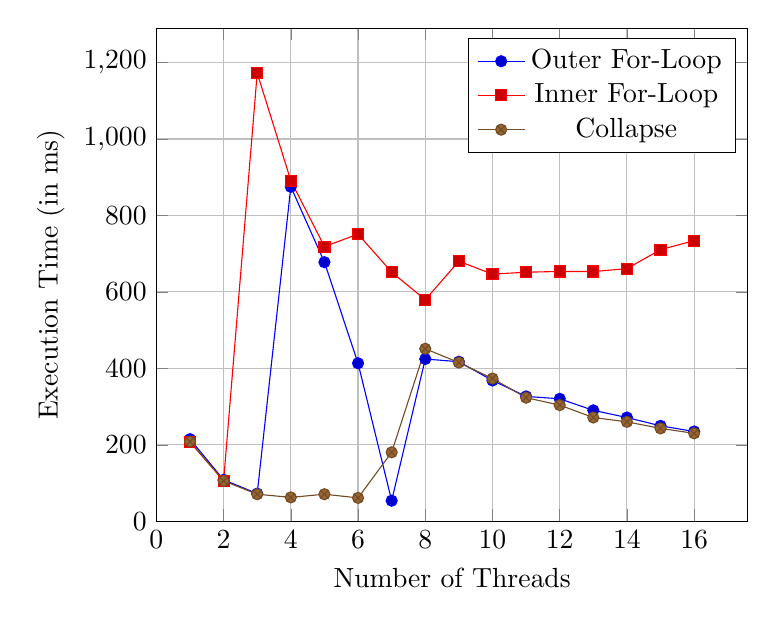
\begin{tikzpicture}
            \begin{axis}[
                title={},
                width=0.75\textwidth,
                xlabel={Number of Threads},
                ylabel={Execution Time (in ms)},
                xmin=0,
                ymin=0,
                grid=major
            ]
                \addplot coordinates {
                    (1,214.884)(2,108.496)(3,72.487)(4,874.89)(5,677.734)(6,413.441)(7,53.8604)(8,424.53)(9,417.405)(10,368.377)(11,326.656)(12,320.394)(13,290.219)(14,271.449)(15,249.741)(16,234.925)
                };
                \addlegendentry{Outer For-Loop}

                \addplot coordinates {
                    (1,207.426)(2,106.252)(3,1172.46)(4,891.04)(5,718.439)(6,751.246)(7,651.642)(8,579.481)(9,680.238)(10,646.528)(11,651.56)(12,653.486)(13,653.193)(14,660.897)(15,710.533)(16,734.047)
                };
                \addlegendentry{Inner For-Loop}       

                \addplot coordinates {
                    (1,208.478)(2,105.691)(3,70.8347)(4,62.5586)(5,70.8706)(6,61.2197)(7,180.496)(8,451.336)(9,415.158)(10,373.54)(11,323.338)(12,303.868)(13,271.512)(14,260.139)(15,242.993)(16,230.13)
                };
                \addlegendentry{Collapse}
            \end{axis}
        \end{tikzpicture}
        \caption{Emboss Performance Tests dice.png}
    \end{figure}
\end{center}

\end{frame}

\begin{frame}
    \frametitle{Emboss - Ergebnisse 3}

    \begin{itemize}
        \item pnglogo-blk.png
        \item 1024 x 768
        \item 516 KB
    \end{itemize}

    \hfill
    \hrule
    \hfill

    \begin{figure}[H]
        \centering
    
        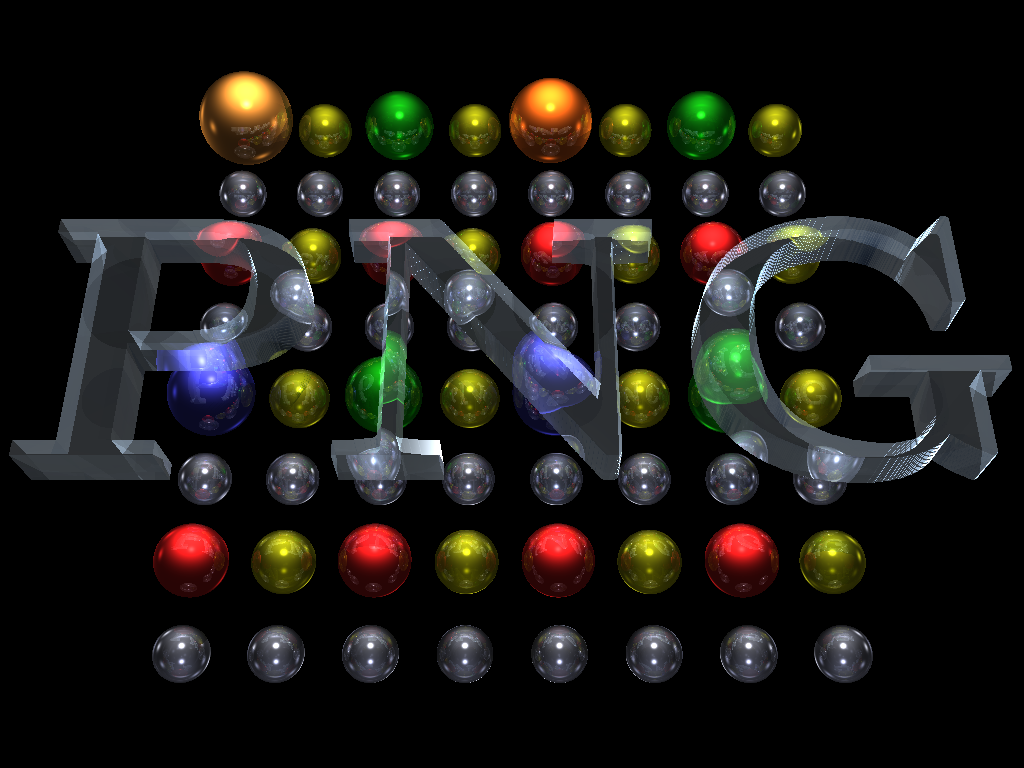
\includegraphics[width=0.30\textwidth]{images/pnglogo-blk.png}
        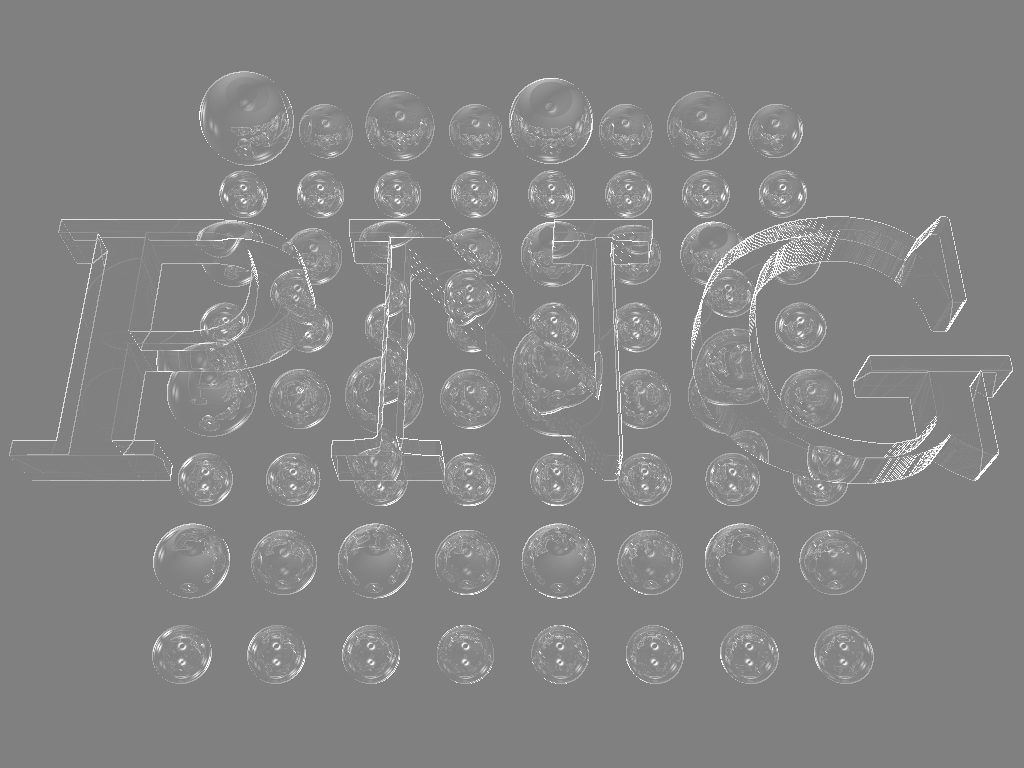
\includegraphics[width=0.30\textwidth]{images/results/emboss-my.pnglogo-blk.png}

        
        \begin{center}
            \caption{Emboss results of self-implemented Algorithm (right)}
        \end{center}

        \label{fig:emboss3}
    \end{figure}
\end{frame}

\begin{frame}
    \frametitle{Emboss - Performance 3}

    \begin{center}
    \begin{figure}[H]
        \centering

        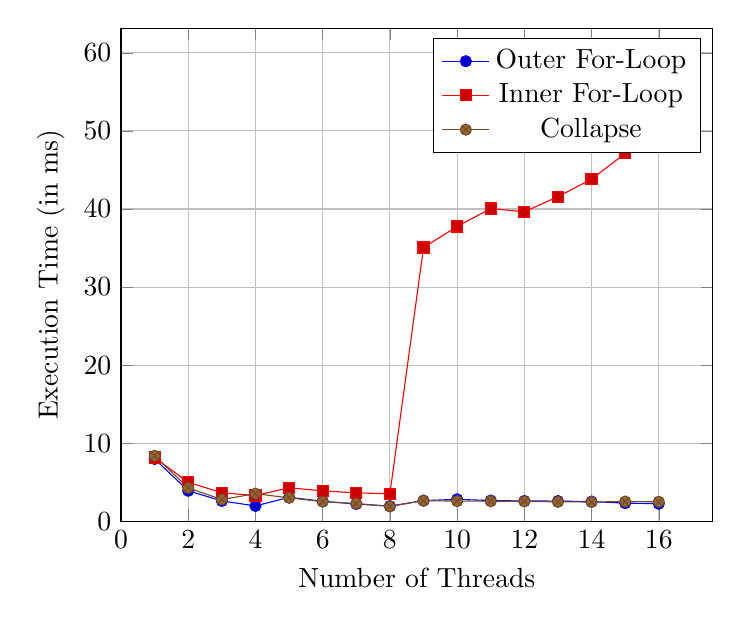
\begin{tikzpicture}
            \begin{axis}[
                title={},
                width=0.75\textwidth,
                xlabel={Number of Threads},
                ylabel={Execution Time (in ms)},
                xmin=0,
                ymin=0,
                grid=major
            ]
                \addplot coordinates {
                    (1,7.98865)(2,3.91065)(3,2.608)(4,1.9658)(5,3.07375)(6,2.5663)(7,2.21405)(8,1.9445)(9,2.64595)(10,2.81395)(11,2.65795)(12,2.60165)(13,2.5888)(14,2.52365)(15,2.3272)(16,2.2523)
                };
                \addlegendentry{Outer For-Loop}

                \addplot coordinates {
                    (1,8.1666)(2,4.98855)(3,3.6625)(4,3.2951)(5,4.29465)(6,3.90035)(7,3.6383)(8,3.53105)(9,35.0564)(10,37.7613)(11,40.0554)(12,39.6329)(13,41.5814)(14,43.8201)(15,47.1202)(16,57.4096)
                };
                \addlegendentry{Inner For-Loop}       

                \addplot coordinates {
                    (1,8.37795)(2,4.27585)(3,2.78925)(4,3.53475)(5,3.008)(6,2.5163)(7,2.269)(8,1.90685)(9,2.64125)(10,2.5832)(11,2.57355)(12,2.55125)(13,2.493)(14,2.47165)(15,2.52675)(16,2.50055)
                };
                \addlegendentry{Collapse}
            \end{axis}
        \end{tikzpicture}
        \caption{Emboss Performance Tests pnglogo-blk.png}
    \end{figure}
\end{center}

\end{frame}